\documentclass[a4paper,12pt]{report}
\usepackage[brazil]{babel} % Língua do documento
\usepackage[utf8]{inputenc} % Codificação do documento
\usepackage{amsmath,amssymb} % Pacotes para matemática
\usepackage{graphicx} % Inclusão de gráficos
\usepackage{hyperref} % Links clicáveis no documento
\usepackage{setspace} % Espaçamento
\usepackage{indentfirst} % Indentar o primeiro parágrafo de cada seção
\usepackage{geometry}
\usepackage{array}
\usepackage{float}
\usepackage{cite}
\usepackage{url}

\setlength{\parindent}{1.25cm} % Tamanho do parágrafo
\setlength{\parskip}{0.2cm} % Espaçamento entre parágrafos
\onehalfspacing % Espaçamento 1,5

\begin{document}

% CAPA
\begin{titlepage}
    \centering
    {\large \textbf{UNIVERSIDADE DE SÃO PAULO - USP}}\\[1cm]
    {\large \textbf{Bacharelado em Estatística e Ciência de Dados}}\\[3cm]
    {\large \textbf{Gustavo Augusto dos Santos}}\\[1cm]
    {\large \textbf{Kalebi Henrique Silva de Carvalho}}\\[1cm]
    {\large \textbf{Leonan Nelson da Silva Natal}}\\[1cm]
    {\Large \textbf{Tendências Sazonais e Gestão de Crises: Um Estudo sobre Surto Endêmico de COVID-19 em São Carlos Pós Lockdown}}\\[3cm]
    \vfill
    {\large \textbf{São Carlos - SP}}\\
    {\large \textbf{2024}}
\end{titlepage}

% FOLHA DE ROSTO
\begin{titlepage}
    \centering
     {\large \textbf{Gustavo Augusto dos Santos}}\\[1cm]
    {\large \textbf{Kalebi Henrique Silva de Carvalho}}\\[1cm]
    {\large \textbf{Leonan Nelson da Silva Natal}}\\[1cm]
    {\Large \textbf{Tendências Sazonais e Gestão de Crises: Um Estudo sobre Surto Endêmico de COVID-19 em São Carlos Pós Lockdown}}\\[3cm]
    \vfill
\begin{flushright}
    \begin{minipage}{0.5\textwidth}
        \large{\textbf{Trabalho da disciplina de \textbf{Metodologia Científica I} apresentado à \textbf{Universidade de São Paulo - USP} como requisito parcial para a obtenção de aprovação na referida disciplina.
}}\\[2cm]
        \large{Docente: \textbf{Prof. Dr. Mário de Castro Andrade Filho }}
    \end{minipage}
\end{flushright}
    \vfill
    {\large \textbf{São Carlos-SP}}\\
    {\large \textbf{2024}}
\end{titlepage}

% ABSTRACT
\chapter*{Resumo}
\addcontentsline{toc}{chapter}{Resumo}
Com o término do período classificado como pandêmico da COVID-19, a transição para uma fase endêmica apresenta novos desafios e demandas para a saúde pública. Diante disso, torna-se essencial realizar estudos focados na contenção e caracterização de surtos endêmicos de SARS-CoV-2. Este trabalho propõe identificar padrões sazonais relacionados a eventos geradores de crises regionais no município de São Carlos. Os dados foram analisados utilizando técnicas estatísticas e inferenciais, tais como testes de hipóteses e análises gráficas, por meio de frameworks Python (Pandas e Matplotlib). Espera-se que as análises quantitativas resultem em padrões qualitativos para a mensuração de possíveis crises endêmicas.

\vspace{0.5cm}
\noindent \textbf{Palavras-Chave}: COVID-19, Endêmico, Saúde Pública, Padrões Sazonais, Crises Regionais, São Carlos, Análise Exploratória de Dados, Python.

\chapter*{Abstract}
\addcontentsline{toc}{chapter}{Abstract}
 With the end of the period classified as a COVID-19 pandemic, the transition to an endemic phase presents new challenges and demands for public health. Therefore, it is essential to carry out studies focused on the containment and characterization of endemic outbreaks of SARS-CoV-2. This paper aims to identify seasonal patterns related to events that generate regional crises in the city of São Carlos. Data were analyzed using statistical and inferential techniques, such as hypothesis testing and graphical analysis, using Python frameworks (Pandas and Matplotlib). It is expected that quantitative analyses will result in qualitative standards for the measurement of possible endemic crises. 

\vspace{0.5cm}
\noindent \textbf{Keywords}:COVID-19, Endemic, Public Health, Seasonal Patterns, Regional Crises, San Carlos, Exploratory Data Analysis, Python. 

% SUMÁRIO
\tableofcontents

% INTRODUÇÃO
\chapter*{Introdução}
\addcontentsline{toc}{chapter}{Introdução}
\label{chap:introducao}
A observação contínua de várias doenças ao longo do tempo tem revelado que variações sazonais na incidência são comuns para infecções agudas. Por exemplo, a gripe espanhola de 1918-1919 mostrou padrões sazonais evidentes \cite{taubenberger2006} , e estudos subsequentes sobre o vírus da gripe continuam a identificar flutuações sazonais regulares na incidência da doença. Da mesma forma, a dengue exibe picos sazonais que estão intimamente ligados a fatores climáticos e ambientais \cite{johansson2009}.

A compreensão da sazonalidade na dinâmica de transmissão da COVID-19 ainda não é completa, devido não apenas às mudanças climáticas significativas, mas também à capacidade do patógeno de prosperar em diferentes ambientes.

A dificuldade em estabelecer uma dinâmica sazonal clara para a COVID-19 é evidente, dada a complexidade dos dados disponíveis\cite{andrade2022sazonalidade}.

No entanto, se confirmado esse padrão, seria de extrema importância para compreender e mitigar os riscos e os fatores determinantes da transmissão do SARS-CoV-2, contribuindo para o planejamento de estratégias eficazes de controle e prevenção durante crises endêmicas.

Este estudo investigou a hipótese de sazonalidade da COVID-19 no município de São Carlos-SP, nos anos de 2022, 2023 e no primeiro semestre de 2024, período em que os níveis de cobertura vacinal da população já são considerados médios a altos.

\chapter*{Objetivos}
\addcontentsline{toc}{chapter}{Objetivos}
\label{chap:objetivos}
Este trabalho tem como objetivo central investigar os padrões sazonais associados aos eventos geradores de crises endêmicas no contexto pós-pandêmico da COVID-19, focando no município de São Carlos. Com a transição da COVID-19 para uma fase endêmica, emergem novos desafios e demandas significativas para a saúde pública, especialmente na contenção e caracterização de surtos locais do SARS-CoV-2.

O estudo utilizará técnicas estatísticas avançadas e análises inferenciais, incluindo visualizações gráficas, empregando frameworks em Python como Pandas e Matplotlib. Através dessas metodologias, pretende-se identificar e quantificar padrões qualitativos que possam indicar a ocorrência e a intensidade de crises endêmicas no município.

Ao final, espera-se que os resultados obtidos forneçam insights críticos para a gestão de saúde pública local, contribuindo para estratégias mais eficazes de monitoramento, prevenção e resposta a surtos endêmicos de SARS-CoV-2, consolidando assim a base científica necessária para enfrentar futuras emergências de saúde.

\chapter*{Metodologia}
\addcontentsline{toc}{chapter}{Metodologia}
\label{chap:metodologia}

\section*{Coleta de Dados}
\addcontentsline{toc}{section}{Coleta de Dados}
Os dados foram obtidos através do site oficial de monitoramento da COVID-19\cite{brasilcovid}, especificamente de registros semanais de notificações de casos novos e óbitos. Os dados abrangem as semanas epidemiológicas dos anos de 2022, 2023 e 2024.

\section*{Organização dos Dados}
\addcontentsline{toc}{section}{Organização dos Dados}
Os dados foram organizados em um formato Data Frame utilizando-se a biblioteca Pandas do Python. Cada entrada no DataFrame continha informações sobre a semana epidemiológica, o ano correspondente, o número de casos novos notificados e o número de óbitos novos notificados.

\section*{Análise Descritiva}
\addcontentsline{toc}{section}{Análise Descritiva}
A análise descritiva dos dados foi conduzida utilizando tabelas resumo de frequência. Essas tabelas fornecem uma visão geral da distribuição dos casos novos e óbitos notificados ao longo das semanas epidemiológicas.

\section*{Visualização dos Dados}
\addcontentsline{toc}{section}{Visualização dos Dados}
Foram criados gráficos de séries temporais para facilitar a visualização dos padrões de notificação ao longo do tempo:

Gráficos de Casos Novos Notificados: Os casos novos notificados foram plotados para cada semana epidemiológica, com as séries separadas por ano e diferenciadas por cores.

Gráficos de Casos Acumulados: Para entender a progressão ao longo do tempo, os casos acumulados foram calculados e plotados, mostrando o total acumulado de casos semana a semana.

Gráfico da Média Móvel :Os casos foram analisados por meio do emprego de uma técnica de média móvel, utilizada para suavizar os dados, proporcionando uma visualização mais clara das tendências e padrões que emergem ao longo do período analisado.

\section*{Ferramentas Utilizadas}
\addcontentsline{toc}{section}{Ferramentas Utilizadas}
As seguintes ferramentas e bibliotecas foram utilizadas para a análise e visualização dos dados:

\begin{itemize}
    \item Python: A linguagem de programação utilizada para todas as etapas de manipulação e análise de dados.

    \item Pandas: Biblioteca utilizada para a manipulação e transformação dos dados.

    \item Matplotlib: Biblioteca utilizada para a criação dos gráficos de séries temporais.

    \item Google Sheets: Plataforma utilizada para formatação das tabelas de frequências
\end{itemize}


\chapter*{Resultados e Discussão}
\addcontentsline{toc}{chapter}{Resultados e Discussão}
\label{chap:resultados}
Esta seção apresenta os principais resultados obtidos da análise dos dados epidemiológicos, com foco na visualização dos padrões de notificação ao longo do tempo. Para facilitar a interpretação dos dados, foram criados gráficos de séries temporais que permitem uma análise detalhada das tendências observadas.

\begin{table}[ht]
    \centering
    \centering
    \begin{tabular}{|>{\centering\arraybackslash}m{5cm}|>{\centering\arraybackslash}m{2cm}|>{\centering\arraybackslash}m{2cm}|>{\centering\arraybackslash}m{2cm}|>{\centering\arraybackslash}m{2cm}|}
        \hline
        Ano 2022 & Frequência Absoluta & Frequência Acumulada & Frequência Percentual & Frequência Percentual Acumulada \\
        \hline
        Semana  01 - Semana  04 & 129 &  129 & 01,23\% & 01,23\% \\
        Semana  05 - Semana  08 & 575 &  704 & 29,50\% & 30,73\% \\
        Semana  09 - Semana  12 & 294 &  998 & 15,08\% & 45,82\% \\
        Semana  13 - Semana  16 & 040 & 1.038& 02,05\% & 47,87\% \\
        Semana  17 - Semana  20 & 082 & 1.120& 04,21\% & 52,08\% \\
        Semana  21 - Semana  24 & 287 & 1.407& 14,73\% & 66,80\% \\
        Semana  25 - Semana  28 & 243 & 1.650& 12,47\% & 79,27\% \\
        Semana  29 - Semana  32 & 165 & 1.815& 08,47\% & 87,74\% \\
        Semana  33 - Semana  36 & 143 & 1.958& 07,34\% & 95,07\% \\
        Semana  37 - Semana  40 & 029 & 1.987& 01,49\% & 96,56\% \\
        Semana  41 - Semana  44 & 005 & 1.992& 00,26\% & 96,82\% \\
        Semana  45 - Semana  48 & 015 & 2.007& 00,77\% & 97,59\% \\
        Semana  49 - Semana  52 & 047 & 2.054& 02,41\% &100,00\% \\
        \hline
            Total              & 2.054 & 2.054  & 100,00\% & 100,00\%  \\           
        \hline
    \end{tabular}
    \caption{Tabela de Frequências para o Ano de 2022}
    \label{tab:frequencias_2022}
\end{table}

\begin{figure}[H]
    \centering
    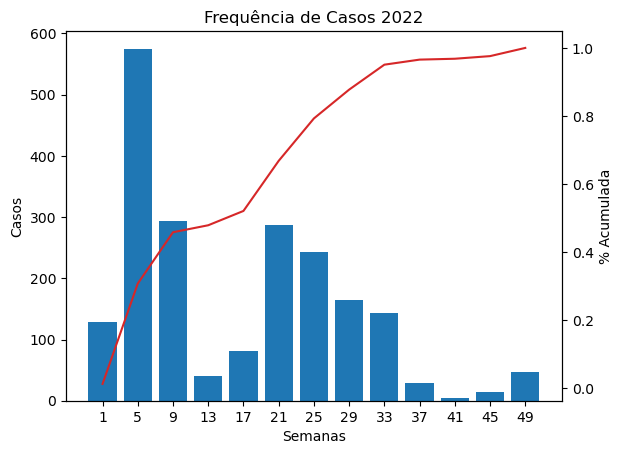
\includegraphics[width=0.85\linewidth]{Frequência 2022.png}
    \caption{Frequência 2022}
    \label{fig:enter-label}
\end{figure}

No ano de 2022, a cidade de São Carlos registrou um pico de 575 casos de COVID-19 entre a 5ª e a 8ª semana. Durante as semanas do meio do ano, quando o clima é mais frio, os casos se mantiveram em alta, resultando em 95\% dos casos anuais ocorrendo até a 36ª semana epidemiológica. Em contraste, em 2023, houve dois períodos de alta nos casos: um no início do ano e outro no final. Entre a 17ª e a 36ª semana, o número de casos permaneceu abaixo de 100 por mês, contrariando a tendência observada em 2022. 
No período avaliado, a cidade de São Carlos registrou uma significativa concentração de casos de COVID-19 nas 12 primeiras semanas do ano (fig. 3). Esse período inicial foi responsável por 45,82\% e 48,94\% dos casos em 2022 e 2023, respectivamente, destacando um padrão consistente de alta incidência nos primeiros meses do ano. Em 2024, a cidade acumulou até a 12ª semana 561 casos de COVID-19, um valor menor que o dos anos anteriores. No entanto, devido ao alto número de casos entre a 13ª e a 15ª semana, os dados de 2024 já se aproximam dos padrões observados nos anos anteriores.
 

\begin{table}[ht]
    \centering
    \begin{tabular}{|>{\centering\arraybackslash}m{5cm}|>{\centering\arraybackslash}m{2cm}|>{\centering\arraybackslash}m{2cm}|>{\centering\arraybackslash}m{2cm}|>{\centering\arraybackslash}m{2cm}|}
        \hline
        Ano 2023 & Frequência Absoluta & Frequência Acumulada & Frequência Percentual & Frequência Percentual Acumulada \\
        \hline
        Semana  01 - Semana  04 & 473 &  473 & 18,24\% & 18,24\% \\
        Semana  05 - Semana  08 & 437 &  910 & 16,85\% & 35,09\% \\
        Semana  09 - Semana  12 & 359 & 1.269& 13,84\% & 48,94\% \\
        Semana  13 - Semana  16 & 240 & 1.509& 09,26\% & 58,20\% \\
        Semana  17 - Semana  20 & 026 & 1.535& 01,00\% & 59,20\% \\
        Semana  21 - Semana  24 & 053 & 1.588& 02,04\% & 61,24\% \\
        Semana  25 - Semana  28 & 030 & 1.618& 01,16\% & 62,40\% \\
        Semana  29 - Semana  32 & 015 & 1.633& 00,58\% & 62,98\% \\
        Semana  33 - Semana  36 & 045 & 1.678& 01,74\% & 64,71\% \\
        Semana  37 - Semana  40 & 305 & 1.983& 11,76\% & 76,48\% \\
        Semana  41 - Semana  44 & 267 & 2.250& 10,30\% & 86,77\% \\
        Semana  45 - Semana  48 & 230 & 2.480& 08,87\% & 95,64\% \\
        Semana  49 - Semana  52 & 113 & 2.593& 04,36\% &100,00\% \\
        \hline
            Total              & 2.593 &  2.593 & 100,00\% & 100,00\% \\           
        \hline
    \end{tabular}
    \caption{Tabela de Frequências para o Ano de 2023}
    \label{tab:frequencias_2023}
\end{table}

\begin{figure}[H]
    \centering
    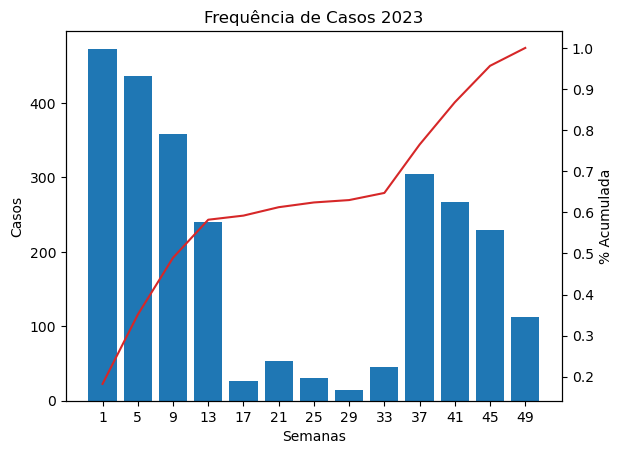
\includegraphics[width=0.85\linewidth]{Frequência 2023.png}
    \caption{Frequência 2023}
    \label{fig:enter-label}
\end{figure}


\begin{table}[H]
    \centering
    \begin{tabular}{|>{\centering\arraybackslash}m{5cm}|>{\centering\arraybackslash}m{2cm}|>{\centering\arraybackslash}m{2cm}|>{\centering\arraybackslash}m{2cm}|>{\centering\arraybackslash}m{2cm}|}
        \hline
        Ano 2024 & Frequência Absoluta & Frequência Acumulada & Frequência Percentual & Frequência Percentual Acumulada \\
        \hline
        Semana  01-Semana  04 & 122 &  122 & 11,23\% & 11,23\% \\
        Semana  05-Semana  08 & 397 &  519 & 36,56\% & 47,79\% \\
        Semana  09-Semana  12 & 042 &  561 & 03,87\% & 51,66\% \\
        Semana  13-Semana  16 & 525 & 1.086& 48,34\% &100,00\% \\
        \hline
            Total              & 1.086 &  1.086 & 100,00\% & 100,00\% \\           
        \hline
    \end{tabular}
    \caption{Tabela de Frequências para o Ano de 2024}
    \label{tab:frequencias_2024}
\end{table}

\begin{figure}[H]
    \centering
    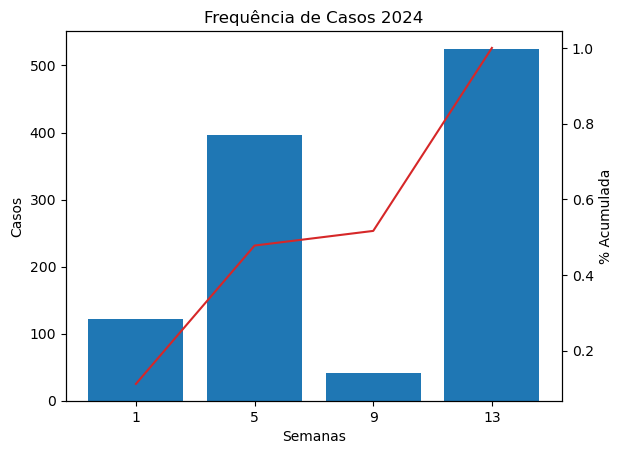
\includegraphics[width=1\linewidth]{Frequência 2024.png}
    \caption{Frequência 2024}
    \label{fig:enter-label}
\end{figure}

\begin{figure}[H]
    \centering
    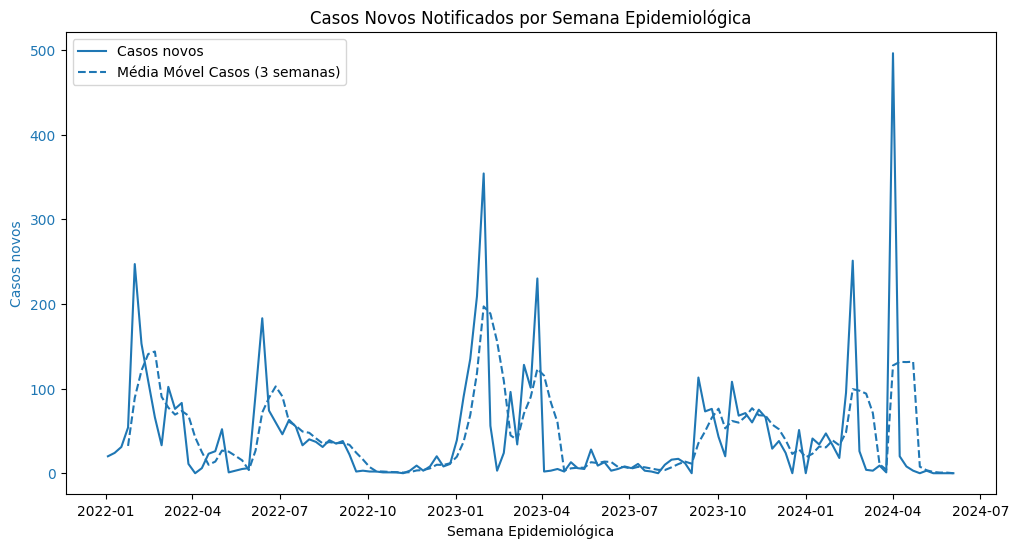
\includegraphics[width=1\linewidth]{Casos Novos notificados por semana epidemiologica.png}
    \caption{Casos Novos Notificados por Semana Epidemiológica}
\end{figure}


\begin{figure}[htbp]
    \centering
    \begin{minipage}[b]{0.45\textwidth}
        \centering
        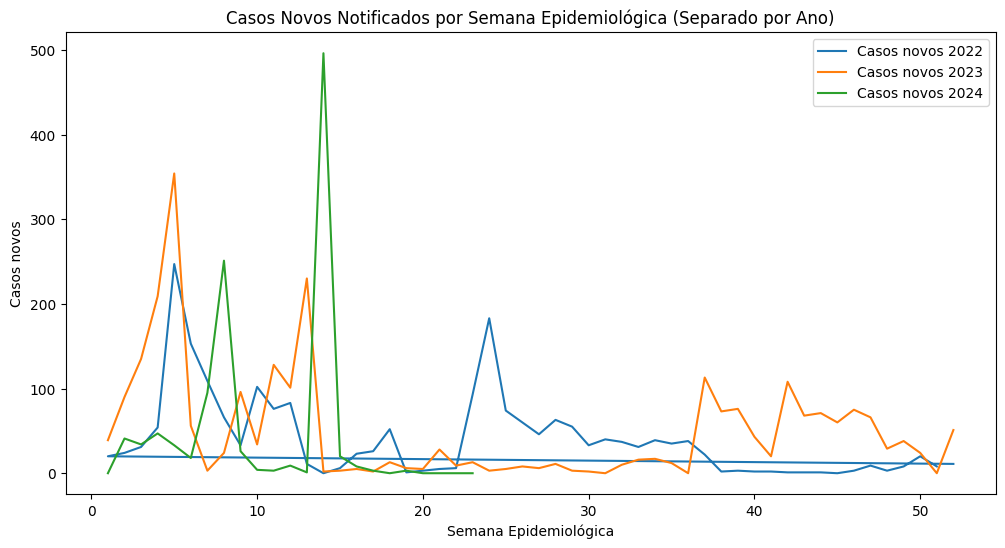
\includegraphics[width=\textwidth]{Casos Novo separados por ano.png} 
        \caption{Casos Novos Notificados por Semana Epidemiológica(Separado por Ano)}
    \end{minipage}
    \hfill
    \begin{minipage}[b]{0.45\textwidth}
        \centering
        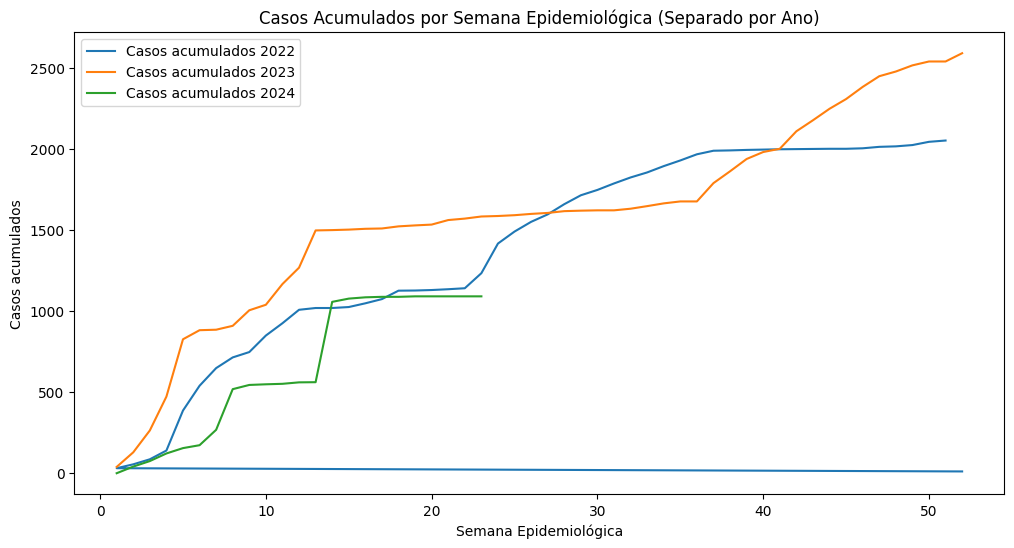
\includegraphics[width=\textwidth]{Casos Acumulados.png}
        \caption{Casos Acumulados por Semana Epidemiológica(Separado por Ano)}
    \end{minipage}
\end{figure}


\footnotetext{\textbf{Obs: Todos os gráficos e tabelas de frequência foram de autoria própria dos autores.}}

No gráfico ilustrado na Figura 4, a linha tracejada representa a aplicação da Média Móvel, uma técnica estatística fundamental na análise de séries temporais. Seu objetivo principal é identificar padrões subjacentes, variações sazonais e mudanças de curto prazo nos dados. A Média Móvel é conhecida por sua capacidade de suavizar flutuações aleatórias, destacando assim as tendências significativas ao longo do tempo.

A essência da Média Móvel reside no cálculo da média de um determinado número de pontos consecutivos em uma série temporal. Esse procedimento ajuda a reduzir o impacto das flutuações aleatórias, permitindo uma melhor visualização das tendências que podem não ser facilmente discerníveis nos dados originais. No caso apresentado, a Média Móvel foi calculada utilizando um período de 3 semanas.

\begin{center}
    \begin{equation}
        \bar{p_i} = \frac{p_{i+1}+ \ldots + p_{i+n}}{n} = \frac{1}{n}\sum_{j=1}^{n}p_{i+j} 
    \end{equation}
\end{center}

\begin{center}
    \begin{equation}
        \bar{p_{i+1}} = \bar{p_i} + \frac{p_{n+i+1}}{n} - \frac{p_{i+1}}{n}
    \end{equation}
\end{center}

Os resultados desta pesquisa demonstram que a COVID-19 apresenta um padrão sazonal claro, com picos de casos nos 3 primeiros meses do ano. Essa sazonalidade pode estar relacionada a fatores climáticos, como temperatura e umidade, que influenciam a viabilidade e a transmissão do vírus, além de períodos de livre circulação e datas comemorativas \cite{xavier2022sazonalidade}.

A compreensão da sazonalidade da COVID-19 é crucial para o planejamento de medidas de saúde pública eficazes. As autoridades podem utilizar os resultados desta pesquisa para direcionar recursos e estratégias de prevenção para os períodos de maior risco da doença.

\section*{Considerações Adicionais:}

\begin{itemize}
    \item É importante destacar que a sazonalidade da COVID-19 pode ser influenciada por outros fatores além dos climáticos, como medidas de controle social e a circulação de novas variantes do vírus.

    \item Mais pesquisas são necessárias para compreender completamente os mecanismos por trás da sazonalidade da COVID-19 e para desenvolver modelos de previsão precisos.
\end{itemize}


\section*{Conclusão}
\addcontentsline{toc}{chapter}{Conclusão}
Com base na análise dos dados dos anos estudados, observamos que aproximadamente metade dos casos de COVID-19 ocorre até a 12ª semana do ano, conforme indicado pelos gráficos de média móvel e de frequências. A concentração desses casos nos primeiros meses pode ser atribuída à presença de feriados significativos como festas de fim de ano, Carnaval e Semana Santa, períodos associados a maiores aglomerações sociais.
Em 2023, os casos permaneceram em baixa durante o meio do ano, tradicionalmente considerados de maior risco para doenças respiratórias, sugerindo que, no Brasil, as aglomerações possam representar um risco maior que o tempo seco e frio.
Embora o gráfico de média móvel não mostre uma tendência clara de crescimento ou decrescimento, o que pode indicar um controle da pandemia de COVID-19, a concentração inicial de casos no começo do ano sublinha a necessidade contínua de precauções e vigilância.





\begin{thebibliography}{99}
\addcontentsline{toc}{chapter}{Referência Bibliográficas}
\bibitem{taubenberger2006}
TAUBENBERGER, Jeffrey K.; MORENS, David M. 1918 Influenza: The Mother of All Pandemics. \textit{Emerging Infectious Diseases}, v. 12, n. 1, p. 15-22, 2006. Disponível em: \url{https://wwwnc.cdc.gov/eid/article/12/1/05-0979_article}. 

\bibitem{johansson2009}
JOHANSSON, Michael A.; CUMMINGS, Derek A. T.; GLASS, Gregory E. Multiyear Climate Variability and Dengue—El Niño Southern Oscillation, Weather, and Dengue Incidence in Puerto Rico, Mexico, and Thailand: A Longitudinal Data Analysis. \textit{PLoS Medicine}, v. 6, n. 11, p. e1000168, 2009. Disponível em: \url{https://journals.plos.org/plosmedicine/article?id=10.1371/journal.pmed.1000168}. 

\bibitem{andrade2022sazonalidade}
ANDRADE, Ion; MOTA, Hugo; OLIVEIRA, Jacyane; MEDEIROS, Flávia. A sazonalidade da Covid-19 em 2021 na região metropolitana de Natal (RN), Brasil. \textit{Revista Diálogos em Saúde Pública}, v. 1, n. 2, p. e000019--e000019, 2022. Disponível em: \url{https://www.researchgate.net/publication/377695427_A_sazonalidade_da_Covid-19_em_2021_na_regiao_metropolitana_de_Natal_RN_Brasil}. 

\bibitem{brasilcovid}
BRASIL. Ministério da Saúde. COVID-19 no Brasil. Disponível em: \url{https://covid.saude.gov.br/}. Acesso em: 17 jun. 2024.

\bibitem{xavier2022sazonalidade}
Xavier, Juliana Meira de Vasconcelos et al. "Sazonalidade climática e doenças das vias respiratórias inferiores: utilização de modelo preditor de hospitalizações pediátricas." \textit{Revista Brasileira de Enfermagem}, v. 75, n. 1, p. e20210680, 2022.

\end{thebibliography}


\end{document}
